\documentclass[border=5pt]{standalone}
\usepackage{amssymb}
\usepackage{amsmath}
\usepackage{tikz}

\usepackage{tikz-inet}
\usepackage{xcolor}

\colorlet{darkred}{red!60!black}
\colorlet{darkblue}{blue!60!black}
\colorlet{darkgreen}{green!60!black}

\usetikzlibrary{positioning, arrows.meta, patterns, calc}
\begin{document}
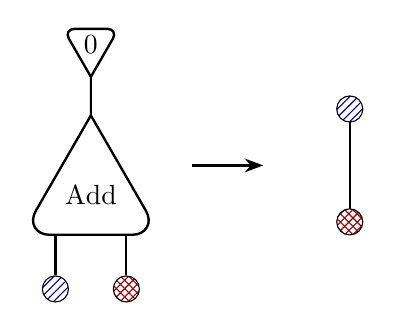
\begin{tikzpicture}[>=Stealth, node distance=0.5cm]
    \begin{scope}[local bounding box=group1]
        
        \inetcell(Add){$\text{Add}$}[U]
        \inetcell[above = of Add.pal](0){$0$}[D]
        % \node (p) [right=of 0.pal] {$\phantom x$};
        % \inetwirefree(Add.right pax)
        % \inetwirefree(Add.left pax)
        \inetwire(0.pal)(Add.pal)
        \node (l) [below = of Add.left pax, draw, circle, pattern color=darkblue, pattern=north east lines] {};
        \node (r) [below = of Add.right pax, draw, circle, pattern color=darkred, pattern=crosshatch] {};
        \draw[thick] (Add.left pax) -- (l);
        \draw[thick] (Add.right pax) -- (r);
    \end{scope}

    \draw[->, thick] (group1.east) ++(0.5,0) -- ++(0.9,0);

    \begin{scope}[shift={(group1.east)}, xshift=2.5cm]
        \matrix[row sep=1em]{
            \node (t) [draw, circle, pattern color=darkblue, pattern=north east lines] {};  \\
            \node (p1) {$\phantom x$}; \\
            \node (b1) [draw, circle, pattern color=darkred, pattern=crosshatch] {}; \\};
            \inetwirecoords(t)(b1)
    \end{scope}
\end{tikzpicture}
\end{document}
